\subsection{Cyber Red Teaming Requirements}
\label{sec:crt}
\glsresetall
% CRT definition
The \gls{rt} definition varies on the domain to which this capability is applied, such as -- command, military, or cyber, as it is discussed in the chapter \ref{sec:crt-work}.
Most common \gls{rt} definition revolves around a small, independent team of highly skilled experts, to provide decision support, alternative analysis and approaches to an existing problem \cite{UK2013} \cite{USJCS2016}.
One definition attempts to present military \gls{crt} as an adversarial-based assessment of own information system vulnerabilities \cite{Brangetto2015}.
Additionally, \gls{rt} is seen as a decision-making supportive element for conducting asymmetric warfare \cite{Longbine2008}.
These definitions are more focused towards supporting decision-making process or providing a specialized assessment of own assets in cyberspace or physically.
It has to be noted, that the \gls{crt} is the \gls{rt} utilizing and performing their assigned tasks mainly within cyberspace and by the use of technology.

% CRT definition weaknesses and re-definition
The aforementioned definitions are directed towards securing and evaluating defender's systems or course of action, but not at affecting the adversary's information systems or decision-making process.
To engage a \gls{crt} in conducting a \gls{cno} within the \gls{rcd} scope, which has the extraterritorial nature, the \gls{crt} has to be structured and possess all the defined qualities and high standards of the \gls{rt}. However, to separate the \gls{rt} activities between internal and external, a concept of \textit{``specialized cyber red teaming''}, directed at the adversary, is proposed.
This thesis addresses the various red team interpretations, use cases, and their applicability, and defines the specialized cyber red team.
\begin{description}
    \label{def:crt}
    \item \textbf{Definition 3.} specialized cyber red team is an independent team of highly skilled experts (1) tasked to perform activities (2) against the adversary's cyber capabilities (3).

    With the essential elements of the definition being:
    \begin{enumerate}
        \item a fully functional and self-sustainable cyber red team operating within the cyberspace;
        \item timely and focused activities against the adversary, for example, conducting the adversarial vulnerability assessment, capability and \gls{tttp} analysis, or execution of computer network operations; and
        \item the cyber red team performed activities being in support of decision-making process, ongoing related operations, or having its own impact delivery.
    \end{enumerate}
\end{description}

% SpecCRT applicability
Such \gls{crt} would be tasked to operate on its own or deliver an effect in support of other activities, such as, cyber-kinetic engagements.
\gls{crt} as such retains the capabilities to operate at any level applicable to deliver the required effect. This could mean operating through kinetic and cyber means to deliver the impact, either directly or indirectly, on the target's cyber or kinetic assets, as long as the execution of operation has the cyber component (Fig. \ref{fig:crt}). As an example, a \gls{crt} might engage in social engineering campaign to gain access to a target server room either physically (e.g., acquiring or copying access cards) or via cyber means (e.g., obtaining remote access password). As well as, for example, gaining remote access to a adversary server room \gls{hvac} system and shutting it down to cause physical effects or damage.
As for the \gls{rt} adversary and threat emulation principle, the \gls{crt} may exercise these approaches to conduct a \textit{false-flag} or \textit{no-flag} operations. Within such operations, the \gls{crt} would pretend and assume the role of another threat actor and adopt its \gls{tttp} to confuse the enemy and make attribution harder or force it to be incorrect.
It has to be pointed out, that the \gls{crt} is a team with suggested size of no more than ten highly skilled experts to keep it balanced and agile, as it is proposed by the UK doctrine \cite{UK2013}. Such small team requires every participant to assume multiple roles to support all of the \gls{crt} operational needs, such as, operational infrastructure planning and deployment, asset acquire, intelligence gathering, \gls{opsec} assurance, targeting, monitoring, and own asset protection. Depending on the available resources and goals, a separate team can be established to support all of the \gls{crt} operational requirements.
Most importantly, a specialized \gls{crt} is the perfect candidate for executing a \gls{cno} within the scope of \gls{rcd}, hence, combining all of the requirements, benefits and restrictions. To create, develop, maintain and evolve such a complete capability the proper resources have to be allocated and invested as early as possible. However, in this thesis, a fully functional specialized \gls{crt} is assumed, and no deeper insights are provided on the assembly, management and its operational requirements, as it is out of the scope of this work.

\begin{figure}[!htb]
    \centering
    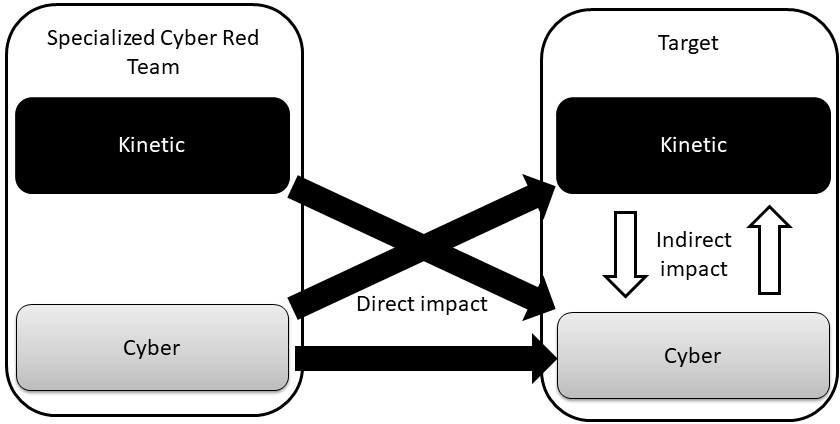
\includegraphics[width=0.8\textwidth]{./img/scrt.jpg}
    \caption{Special cyber red team operation effects}
    \label{fig:crt}
\end{figure}

% CRT requirements
Based on the related work, as presented in the chapter \ref{sec:crt-work} and discussed here, the \gls{crt} has at least the following requirements and characteristics:
\begin{enumerate}
    \item \textbf{Small.} A small team of experts for increased ease of management and agility.
    \item \textbf{Skilled.} Every expert has to be skilled to contribute to the \gls{crt} capability.
    \item \textbf{Specialized.} The team has to self-sustain its independence and operational requirements by providing all the necessary specialized skills.
    \item \textbf{Innovative.} Finding alternative approaches and identifying vulnerabilities in the designated target systems or processes, by applying creativity, critical review and thinking techniques.
    \item \textbf{Highly focused.} Aimed at conducting a specific operation to deliver the designated effect.
    \item \textbf{Targeted.} Persistent in performing precision strikes to complete the assigned task.
    \item \textbf{Asymmetric.} A small team with highly skilled experts having the capability on delivering the maximum possible effect.
    \item \textbf{Adaptive.} Adapting and employing adversarial \gls{tttp} against the target system.
    \item \textbf{Supportive.} Providing support to the ongoing operations, decision-making processes, and operation planning.
    \item \textbf{Timely.} Has to deliver the required effects in the defined time frame.
\end{enumerate}
This is not an exhaustive list and more characteristics could be applicable depending on the particular \gls{crt} organization and tasking specifics.